\chapter{Background}
\label{cha:background}
This chapter describes an architectural overview of the SpiNNaker research, hardware specifications and multicore communication used on my database project.

\section{SpiNNaker Architecture}
\label{sec:spinn_arch}

The basic building block of the SpiNNaker machine is the SpiNNaker Chip Multiprocessor (CMP), a custom designed globally asynchronous locally synchronous (GALS) system \cite{painkras} with 18 ARM968E-S processor nodes (figure \ref{fig:chip_layout}). 
The SpiNNaker chip contains two silicon dies: the SpiNNaker die itself and a 128-MByte SDRAM (Synchronous Dynamic Random Access Memory) die, which is physically mounted on top of the SpiNNaker die and stitch-bonded to it (figure \ref{fig:spinn_dies}) \cite{spinnchip}. The SDRAM serves as local shared memory for the 18 cores within the chip, also utilized for memory based communication \cite{datasheet}. 

\begin{figure}[h]
\centering
\begin{minipage}{.6\textwidth}
  \centering
  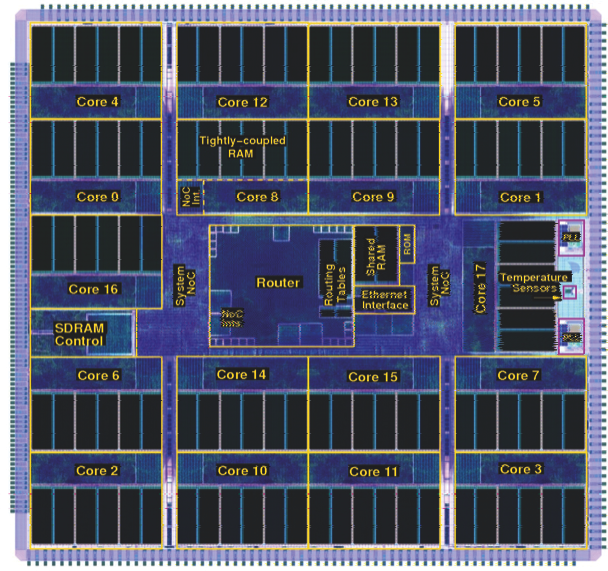
\includegraphics[width=1\linewidth, natwidth=608, natheight=571]{images/chip.png}
  \captionof{figure}{SpiNNaker chip layout}
  \label{fig:chip_layout}
\end{minipage}
\begin{minipage}{.3\textwidth}
  \centering
  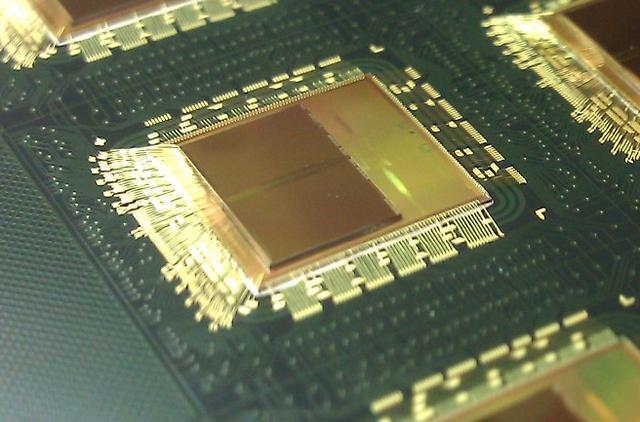
\includegraphics[width=1\linewidth, natwidth=640, natheight=422]{images/spinn_dies.jpg}
  \captionof{figure}{SpiNNaker CMP and SDRAM}
  \label{fig:spinn_dies}
\end{minipage}
\end{figure}

Each ARM core within the chip follows a 32-bit Harvard Architecture, holding a private 32-KB Instruction Tightly Coupled Memory (ITCM) and 64-KB Data Tightly Coupled Memory (DTCM) \cite{painkras}. It has a small peak power consumption of 1-W at the nominal clock frequency of 180-MHz \cite{arm968}.

Figure \ref{fig:4node} shows SpiNN-3, a 4 chip SpiNNaker board with 72 processors, next to figure \ref{fig:48node} (SpiNN-4), composed of 48 chips for a total of 864 processing cores.

\begin{figure}
\centering
\begin{minipage}{.5\textwidth}
  \centering
  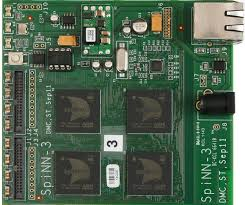
\includegraphics[width=0.4\linewidth, natwidth=245, natheight=205]{images/4node.jpg}
  \captionof{figure}{SpiNN-3}
  \label{fig:4node}
\end{minipage}%
\begin{minipage}{.5\textwidth}
  \centering
  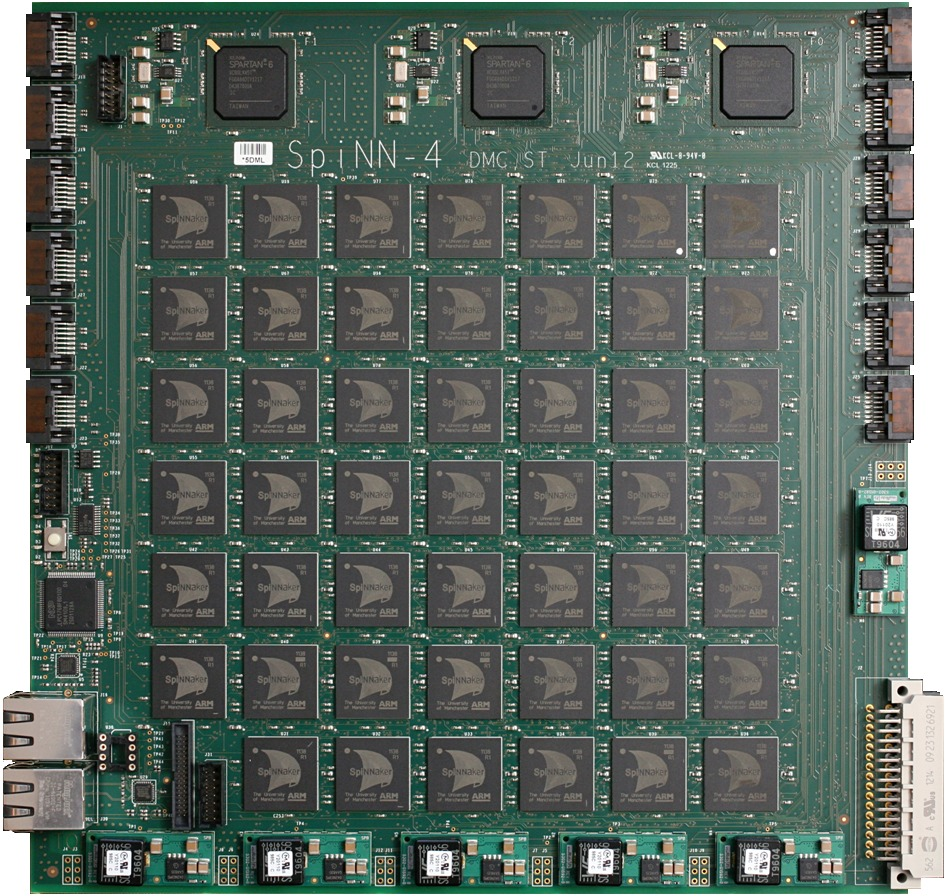
\includegraphics[width=0.9\linewidth, natwidth=945, natheight=896]{images/48node.jpg}
  \captionof{figure}{SpiNN-4}
  \label{fig:48node}
\end{minipage}
\end{figure}

\section{SpiNNaker Communication fabric}
\label{sec:comm_fabric}

Cores on a SpiNNaker board exchange packets through wired connections over a large communication fabric. Each SpiNNaker chip is surrounded by a lightweight, packet-switched asynchronous communication infrastructure \cite{spinnchip}. Packet exchange can be used to transmit information initially private to a core and it is managed under the API's even driven architecture, thus incoming packets issue an interrupt on the receiving core.

There are currently 4 different communication protocols in the event-driven system. It is worth noting that \textbf{none of these protocols guarantee successful delivery of data} and this effect is worsened if there is increased traffic in the communication fabric. Sending a large amount of packets simultaneously is likely to result on packet drops.

\begin{itemize}
\item \textbf{Multicast (MC)}: The MC protocol, originally designed to simulate neural spikes, is used when a single source issues information to multiple destinations (one-to-many), as a fan-out topology \cite{overviewspinn}. The packet contains a 32 bit routing key, used by an external router process to carry out the delivery, and an optional 32 bit payload, both provided at the source.

\item \textbf{Point-to-Point (P2P)}: P2P packets have a single source and a single destination core (one-to-one). Each packet contains a 16-bit source ID, destinarion ID and an optional 32-bit payload \cite{datasheet}.
On top of this layer, the SpiNNaker Datagram Protocol (SDP) was designed to allow transfers of up to 256-bytes of data between two cores, by sending a sequence of P2P packets with payloads \cite{sdp}. SDP can be used to communicate to the \textit{host} machine, wrapped around a larger UDP packet.

\item \textbf{Nearest-neighbour (NN)}: Under the NN protocol, packets issued at a chip will only be delivered to the monitor core on a physically adjacent node \cite{overviewspinn}. NN packets contain a 32-bit payload and a 32-bit address/operation field \cite{datasheet}.

\item \textbf{Fixed-route (FR)}: FR packets use the same mechanism as MC, without a key field. Packets being routed by the contents of a register instead of a routing key. 
\end{itemize}

My database application makes extensive use of the SDP protocol, alongside MC.